\chapter{Conception du système}

\section{Introduction}

La conception est une phase déterminante dans le cycle de vie d'une application. Elle a pour objectif de représenter l'architecture du système et de formaliser les besoins fonctionnels exprimés lors de l'analyse. Elle constitue une étape incontournable pour garantir une mise en œuvre structurée et efficace de la plateforme de gestion des demandes administratives et de matériels du laboratoire IRESCOMATH.

\section{Choix du langage de modélisation}

\subsection{Définition}

Pour modéliser notre application, nous avons choisi le langage UML (Unified Modeling Language). Il s'agit d'un langage de modélisation orienté objet qui permet de représenter visuellement les différents composants d'un système logiciel. UML est largement utilisé pour documenter, spécifier et concevoir les architectures logicielles de manière standardisée.

\subsection{Diagrammes utilisés}

Dans le cadre de la conception de notre projet, nous avons utilisé trois types de diagrammes UML pour illustrer les aspects fonctionnels et structurels du système :

\begin{itemize}
  \item Le diagramme de cas d'utilisation
  \item Le diagramme de séquence
  \item Le diagramme de classes
\end{itemize}

\section{Diagrammes de cas d'utilisation}

\subsection{Présentation des acteurs}

Voici les principaux acteurs identifiés dans notre système :

\begin{itemize}
  \item \textbf{Étudiant-Master} : soumet des demandes de matériels ou administratives.
  \item \textbf{Doctorant} : soumet également des demandes, avec des cas similaires à ceux de l'étudiant master.
  \item \textbf{Enseignant-Chercheur} : peut soumettre des demandes ou valider celles de ses étudiants supervisés.
  \item \textbf{Directeur du laboratoire} : supervise le système et valide les demandes.
  \item \textbf{Administrateur} : gère la plateforme, les comptes utilisateurs, et assure le bon fonctionnement du système. Il peut supprimer un compte.
\end{itemize}


\subsection{Cas d’utilisation }

L’étude des cas d’utilisation a pour objectif de déterminer les attentes fonctionnelles de chaque acteur du système, à travers les interactions qu’il entretient avec la plateforme. Ces cas sont extraits directement de l’analyse des besoins et permettent de structurer l’ensemble des fonctionnalités attendues de l’application de gestion des demandes du laboratoire IReSCoMath.

\paragraph{Cas d’utilisation communs à tous les utilisateurs authentifiés}

Certains cas d’utilisation sont partagés entre plusieurs profils d’utilisateurs : Étudiants-Master, Doctorants, Enseignants-Chercheurs, Directeur du laboratoire et Administrateur. Ces cas génériques assurent l’accès de base à la plateforme.

\begin{itemize}
\item \textbf{S’authentifier} : chaque utilisateur doit passer par une étape d’authentification (identifiant et mot de passe) pour sécuriser l’accès au système. Cette étape est obligatoire avant toute action.
\item \textbf{Se connecter / Créer un compte} : les nouveaux utilisateurs peuvent créer un compte. Une fois la demande validée, ils pourront accéder aux services via une connexion sécurisée.
\item \textbf{Gérer son profil} : chaque membre peut consulter et mettre à jour ses informations personnelles et académiques via un espace dédié.
\end{itemize}

\paragraph{Cas d’utilisation pour les membres (Étudiant-Master, Doctorant, Enseignant-Chercheur)}

Les membres du laboratoire peuvent interagir avec la plateforme principalement pour soumettre et suivre leurs demandes :

\begin{itemize}
\item \textbf{Soumettre une demande} : permet aux membres de générer une demande selon leur rôle (matériel, mission, inscription à un article ou conférence, etc.). Ce cas d’utilisation englobe plusieurs sous-cas selon le type de requête.
\item \textbf{Suivre l’état des demandes} : chaque membre peut visualiser l’état de ses demandes (en attente, acceptée, rejetée, clôturée).
\item \textbf{Recevoir des notifications} : une alerte automatique est déclenchée à chaque mise à jour du statut de la demande ou intervention d’un validateur.
\item \textbf{Compléter une demande} : permet d’enregistrer une demande sans la soumettre immédiatement. L’utilisateur peut y revenir pour la compléter ou la corriger.
\end{itemize}

\paragraph{Cas d’utilisation pour le Directeur du laboratoire}

Le Directeur joue un rôle de validation et de gestion du matériel. Ses responsabilités incluent :

\begin{itemize}
\item \textbf{Gérer les demandes} : permet de valider ou de rejeter les demandes soumises par les membres. Cette action peut être accompagnée de commentaires.
\item \textbf{Gérer les matériels} : permet d’ajouter, modifier ou supprimer un équipement ainsi que de gérer les catégories associées. Ce cas central est détaillé par des cas étendus (<<extend>>).
\item \textbf{Gérer les utilisateurs} : le Directeur peut avoir un rôle secondaire de gestion de certains comptes liés au laboratoire.
\item \textbf{Consulter les bilans et statistiques} : accès à des tableaux de bord consolidés, permettant une vision d’ensemble sur les demandes validées, les dépenses engagées ou les ressources utilisées.
\item \textbf{Modifier les templates de documents imprimés} : personnalisation de modèles utilisés dans les éditions PDF ou les fiches de suivi.
\end{itemize}

\paragraph{Cas d’utilisation pour l’Administrateur}

L’administrateur possède des droits avancés permettant la supervision technique de la plateforme.

\begin{itemize}
\item \textbf{Gérer les utilisateurs} : visualiser l’ensemble des comptes, désactiver ou supprimer un utilisateur.
\item \textbf{Gérer les utilisateurs avec des options avancées} : accès à des options plus poussées comme la réinitialisation de mot de passe, l’activation manuelle de comptes ou l’affectation à des groupes de validation.
\end{itemize}

\subsection{Diagramme de cas d'utilisation global}

En se basant sur le diagramme de cas d’utilisation global, nous identifions les principales fonctionnalités offertes à chaque profil d’utilisateur de la plateforme.

Le \textbf{Directeur du laboratoire} joue un rôle central. Une fois authentifié, il a la capacité de consulter les demandes soumises par les enseignants-chercheurs, doctorants et étudiants master. Il peut valider ou rejeter ces demandes selon leur conformité. Il est également responsable de la gestion du matériel (catégories et équipements) et peut consulter les statistiques et rapports pour un suivi global des activités du laboratoire.

Quant à l'\textbf{Enseignant-Chercheur}, après authentification, il accède aux formulaires de demandes spécifiques comme l’inscription d’articles, les réparations, les missions ou les demandes de matériel. Il peut aussi suivre l'état de ses demandes .

Le \textbf{Doctorant}, après validation de son inscription par le Directeur du Laboratoire, peut se connecter à la plateforme. Il a accès à la gestion de son profil et peut soumettre des demandes diverses telles que les stages, les missions, ou encore le dépôt d’articles. Un système de suivi lui permet d’être informé en temps réel de l’avancement de ses demandes.

De même, l’\textbf{Étudiant-Master} doit soumettre une demande d’adhésion. Une fois celle-ci validée par le directeur du laboratoire, il peut gérer ses informations personnelles et accéder aux formulaires de demandes similaires à ceux du doctorant, selon les permissions qui lui sont attribuées.

Enfin,  l'\textbf{Administrateur} dispose d'un accès complet. Il s’authentifie pour gérer l’ensemble des utilisateurs avec des options avancées comme supprimer un compte.

\begin{figure}[H]
  \centering
  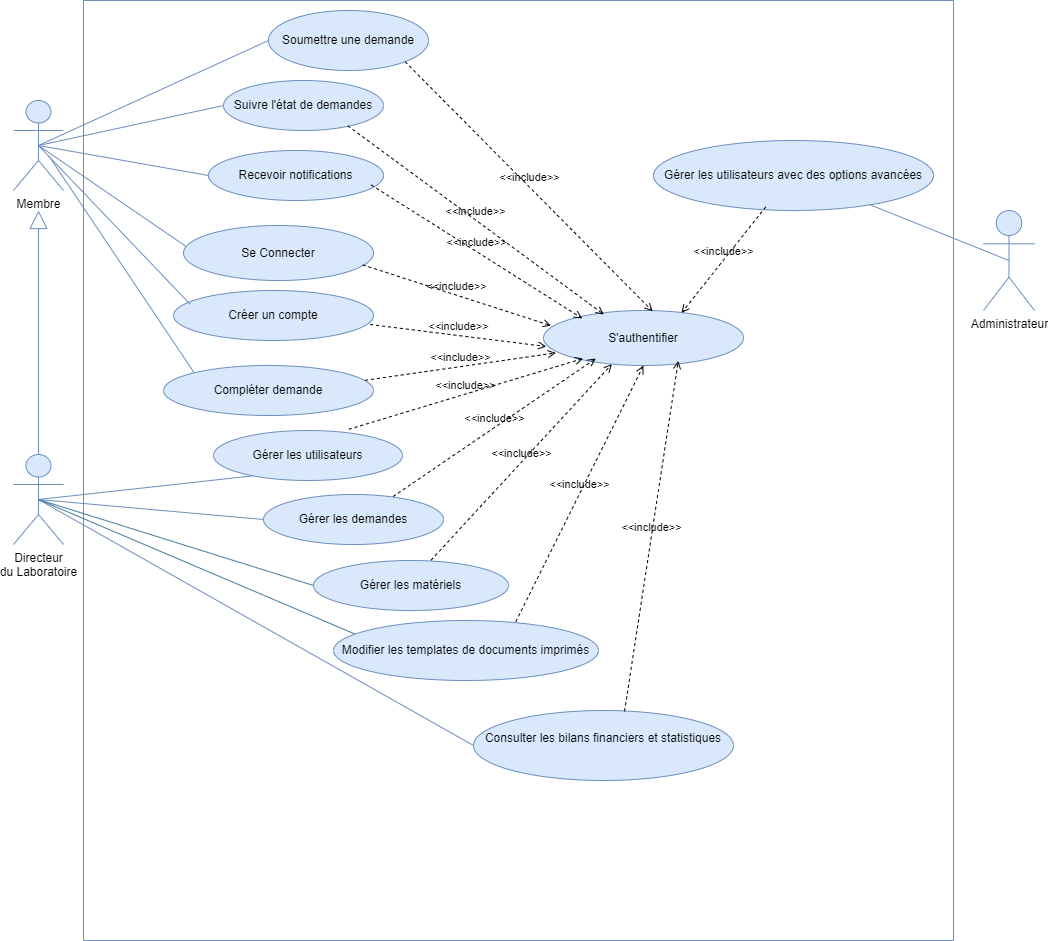
\includegraphics[width=0.9\textwidth]{images/Use_case/Use-Case-Final.drawio.png}
  \caption{Diagramme de cas d'utilisation global du système}
\end{figure}

\subsection{Diagrammes spécifiques par rôle}

\subsubsection{Cas spécifique : Étudiant-Master}
L’Étudiant-Master remplit le formulaire de demande de stage, le soumet au système.

\begin{figure}[H]
  \centering
  \includegraphics[width=0.75\textwidth]{images/Use_case/Cas_spécifique_Etudiant_Master.drawio.png}
  \caption{Diagramme de cas d'utilisation : Étudiant-Master}
\end{figure}

\subsubsection{Cas spécifique : Doctorant}
 Le Doctorant peut soumettre une demande de stage, d’achat ou de prêt de matériel, ainsi qu’une demande d’inscription d’article scientifique.


\begin{figure}[H]
  \centering
  \includegraphics[width=0.75\textwidth]{images/Use_case/Cas_spécifique_Doctorant.drawio.png}
      \caption{Diagramme de cas d'utilisation : Doctorant}
\end{figure}

\subsubsection{Cas spécifique : Enseignant-Chercheur}
L’Enseignant-Chercheur peut soumettre une demande de stage, de matériel (achat ou prêt), d’inscription d’article, de mission, de réparation et maintenance, ainsi que de participation à une conférence nationale.

\begin{figure}[H]
  \centering
  \includegraphics[width=0.75\textwidth]{images/Use_case/Cas_spécifique_Enseignant_chercheur.drawio.png}
  \caption{Diagramme de cas d'utilisation : Enseignant-Chercheur}
\end{figure}

\subsubsection{Cas spécifique : Directeur du laboratoire}

Le Directeur du laboratoire joue un rôle central dans le système, non seulement en tant que valideur final des demandes, mais également en tant que responsable de la gestion stratégique du matériel et du suivi administratif. Ses cas d'utilisation sont regroupés comme suit :

\paragraph{Validation des demandes}

Le Directeur valide les différentes demandes soumises par le membre (achat de matériel, prêt, participation à une conférence nationale, mission, stage, etc.). Il peut soit les approuver, soit les rejeter après vérification.

\begin{figure}[H]
  \centering
  \includegraphics[width=0.75\textwidth]{images/Use_case/Cas_spécifique_Directeur_Demande.drawio.png}
  \caption{Diagramme de cas d'utilisation : Validation des demandes}
\end{figure}



\paragraph{Gestion des matériels}

Le Directeur est également responsable de la gestion des catégories et équipements disponibles dans le laboratoire. Ce cas d'utilisation principal est subdivisé en plusieurs fonctionnalités à travers des extensions :

\begin{figure}[H]
  \centering
  \includegraphics[width=0.85\textwidth]{images/Use_case/Cas_spécifique_Directeur_materiels.drawio.png}
  \caption{Diagramme de cas d'utilisation : Gestion des matériels avec extensions}
\end{figure}

Les fonctionnalités associées sont :
\begin{itemize}
  \item \textbf{Ajout / Modification / Suppression d'une catégorie de matériel}
  \item \textbf{Ajout / Modification / Suppression d'un équipement}
  \item \textbf{Consultation du stock}
\end{itemize}

\subsubsection{Cas spécifique : Administrateur}
L’Administrateur peut gérer les utilisateurs avec des options avancées, telles que la suppression d’un compte utilisateur.

\begin{figure}[H]
  \centering
  \includegraphics[width=0.75\textwidth]{images/Use_case/Cas_spécifique_Administrateur.drawio.png}
  \caption{Diagramme de cas d'utilisation : Administrateur (gestion avancée des utilisateurs)}
\end{figure}

\section{Diagrammes de séquence}

The séquence diagram is the graphical representation of the interactions between the actors and the system according to a chronological order in the UML formulation. On montre ces interactions dans le cadre d'un scénario d'un diagramme des cas d'utilisation. Le but est de décrire comment se déroulent les actions entre les acteurs ou les objets et le système. Voici les diagrammes de séquences des principales fonctionnalités de notre solution.

\subsection{Diagramme de séquence « Validation d'une demande d'adhésion par le Directeur »}

\textbf{Acteur principal :} Directeur du laboratoire \\
\textbf{Objectif :} Valider ou refuser une demande d'inscription soumise par un utilisateur.

\textbf{Scénario principal :}
\begin{enumerate}
  \item Le directeur accède à la liste des demandes.
  \item Il clique sur \texttt{Valider} ou \texttt{Refuser}.
  \item Le frontend envoie une requête \texttt{POST /validate/validate-request}.
  \item Le backend met à jour le statut de la demande dans la base de données.
  \item Le backend envoie un mail à l'utilisateur selon la décision.
\end{enumerate}

\textbf{Scénario alternatif :}
\begin{itemize}
  \item Dans le cas où une erreur est rencontrée, elle est renvoyée avec le code et le message appropriés vers le frontend qui va l'afficher.
\end{itemize}

\begin{figure}[H]
  \centering
  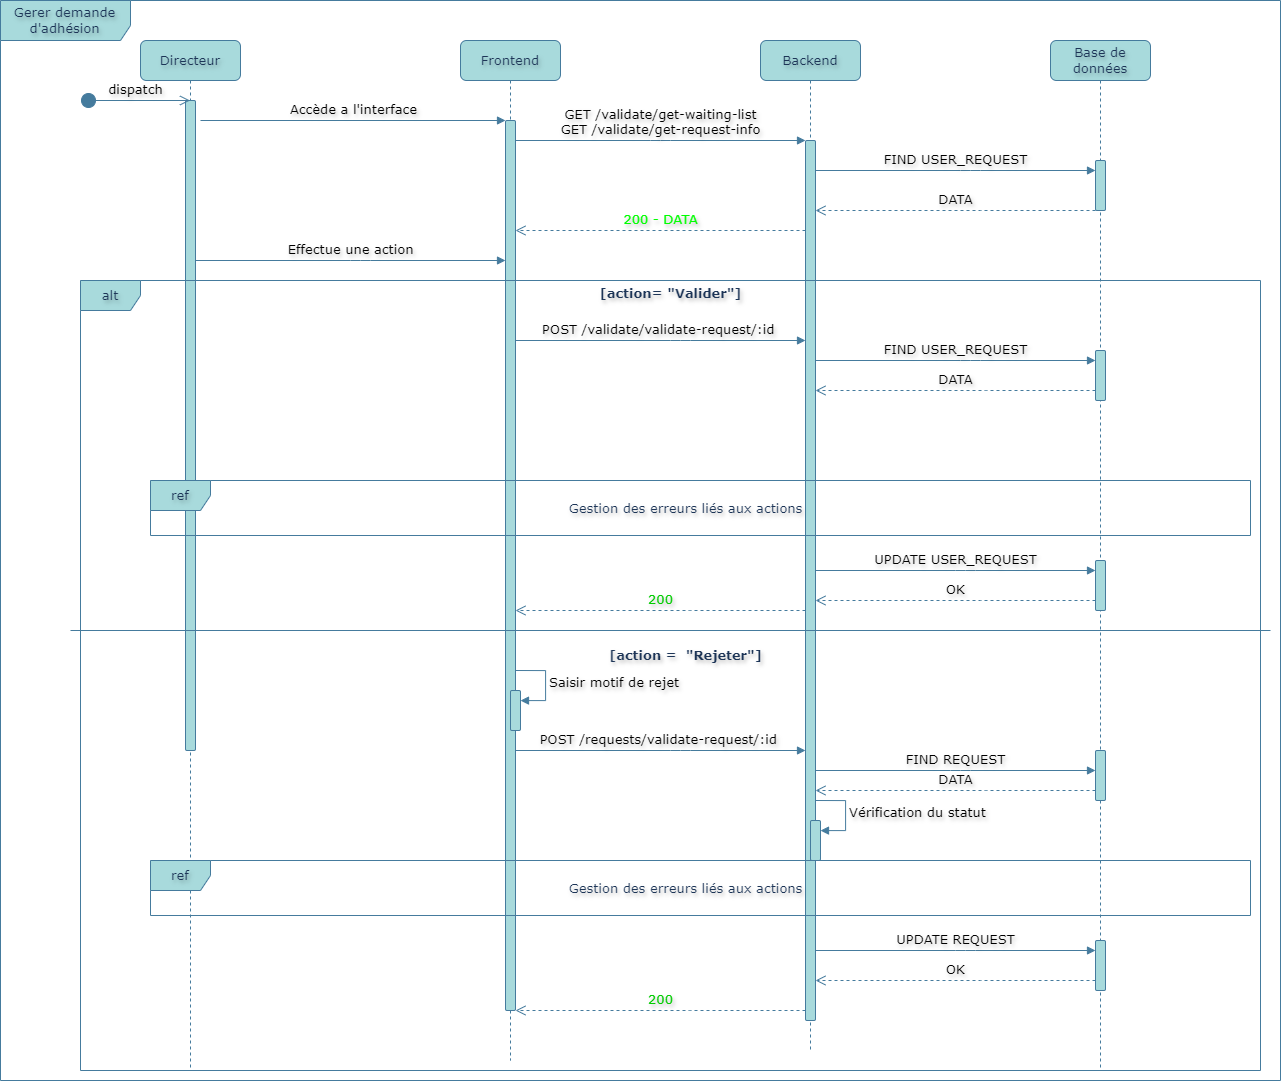
\includegraphics[width=0.95\textwidth]{images/diagramme_de_sequence/gestion_adhesion.png}
  \caption{Diagramme de séquence – Gestion des demandes d'adhésion}
\end{figure}

\begin{figure}[H]
  \centering
  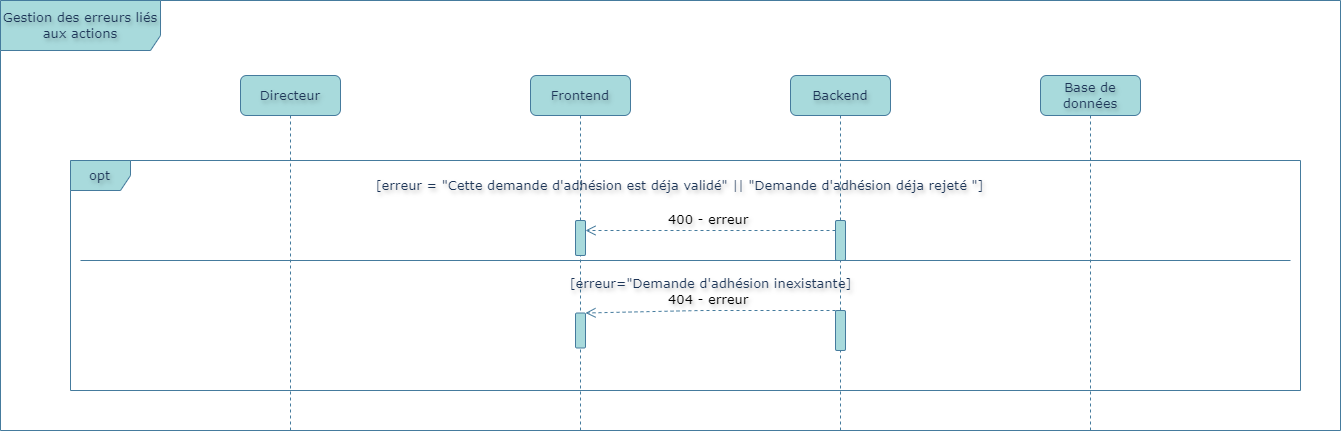
\includegraphics[width=0.95\textwidth]{images/diagramme_de_sequence/gestion_des_erreurs.png}
  \caption{Diagramme de séquence – Gestion des erreurs}
\end{figure}

\subsection{Diagramme de séquence « Soumission d'une demande »}

\textbf{Acteur principal :} Membre validé \\
\textbf{Objectif :} Soumettre une demande.

\textbf{Scénario principal :}
\begin{enumerate}
  \item L'utilisateur accède à l'interface.
  \item Il saisit les informations demandées dans le formulaire.
  \item Le frontend envoie une requête \texttt{POST /requests/\{type\_requests\}}, où \texttt{\{type\_requests\}} représente le type de la requête.
  \item Le backend vérifie la validité des données :
  \begin{itemize}
    \item Si les données sont valides, il crée la requête et retourne un message de succès.
    \item Si les données sont invalides, il retourne un message d'erreur.
  \end{itemize}
  \item Le frontend affiche à l'utilisateur le message de succès ou d'erreur retourné par le backend.
\end{enumerate}

\begin{figure}[H]
  \centering
  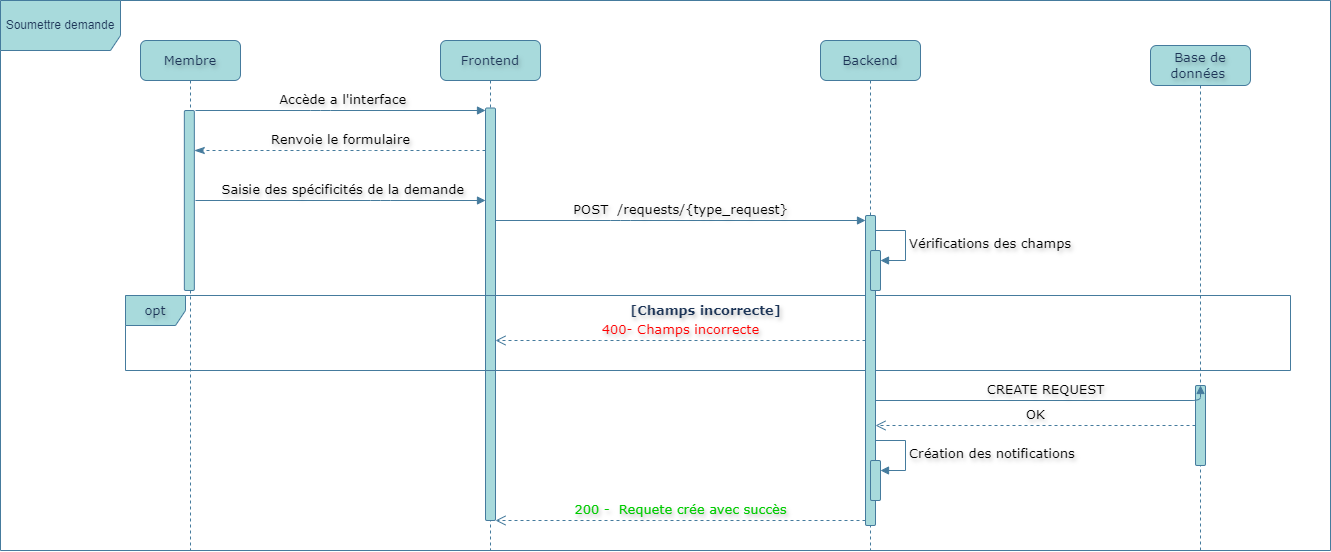
\includegraphics[width=0.95\textwidth]{images/diagramme_de_sequence/soumettre_demande.drawio.png}
  \caption{Diagramme de séquence – Soumission des demandes}
\end{figure}

\subsection{Diagramme de séquence « Gestion des demandes par le directeur »}

\textbf{Acteur principal :} Directeur \\
\textbf{Objectif :} Gérer les demandes (validation, rejet, clôture) soumises par les membres.

\textbf{Scénario principal :}
\begin{enumerate}
  \item Le directeur accède à l'interface de gestion des demandes.
  \item Le frontend récupère et affiche les informations relatives aux demandes en effectuant les requêtes suivantes :
  \begin{itemize}
      \item \texttt{GET /requests/get-all-requests} : obtenir toutes les demandes
      \item \texttt{GET /requests/get-requests/:user\_id} : obtenir les demandes d'un utilisateur spécifique
      \item \texttt{GET /requests/get-request/:request\_id} : obtenir les détails d'une demande spécifique
  \end{itemize}
  \item Le directeur sélectionne une demande et choisit l'action à effectuer :
  
  \textbf{Action : Validation ou Rejet}
  \begin{itemize}
      \item Le frontend envoie une requête \texttt{POST /requests/approve-request/:id} au backend avec l'identifiant de la demande et le statut souhaité (approuvé/rejeté).
      \item Le backend recherche la demande dans la base de données et vérifie son statut actuel.
      \item \textbf{Cas d'erreur :} Si la demande n'existe pas ou si son statut ne permet pas la modification, le backend retourne un code d'erreur avec un message explicatif. Le frontend affiche ce message au directeur.
      \item \textbf{Cas de succès :} Le backend met à jour le statut de la demande, enregistre la modification et envoie une notification au membre concerné.
      \item Le backend retourne un code \texttt{200} avec un message de confirmation. Le frontend affiche un message de succès au directeur.
  \end{itemize}

  \textbf{Action : Clôture}
  \begin{itemize}
      \item Le frontend envoie une requête \texttt{POST /requests/close-request/:id} au backend avec l'identifiant de la demande.
      \item Le backend recherche la demande dans la base de données et vérifie que son statut permet la clôture.
      \item \textbf{Cas d'erreur :} Si la demande ne peut pas être clôturée (statut incompatible, demande inexistante), le backend retourne un code d'erreur approprié. Le frontend affiche le message d'erreur au directeur.
      \item \textbf{Cas de succès :} Le backend marque la demande comme clôturée, enregistre l'action et notifie le membre demandeur.
      \item Le backend retourne un code \texttt{200} avec confirmation. Le frontend affiche un message de succès au directeur.
  \end{itemize}
\end{enumerate}

\begin{figure}[H]
  \centering
  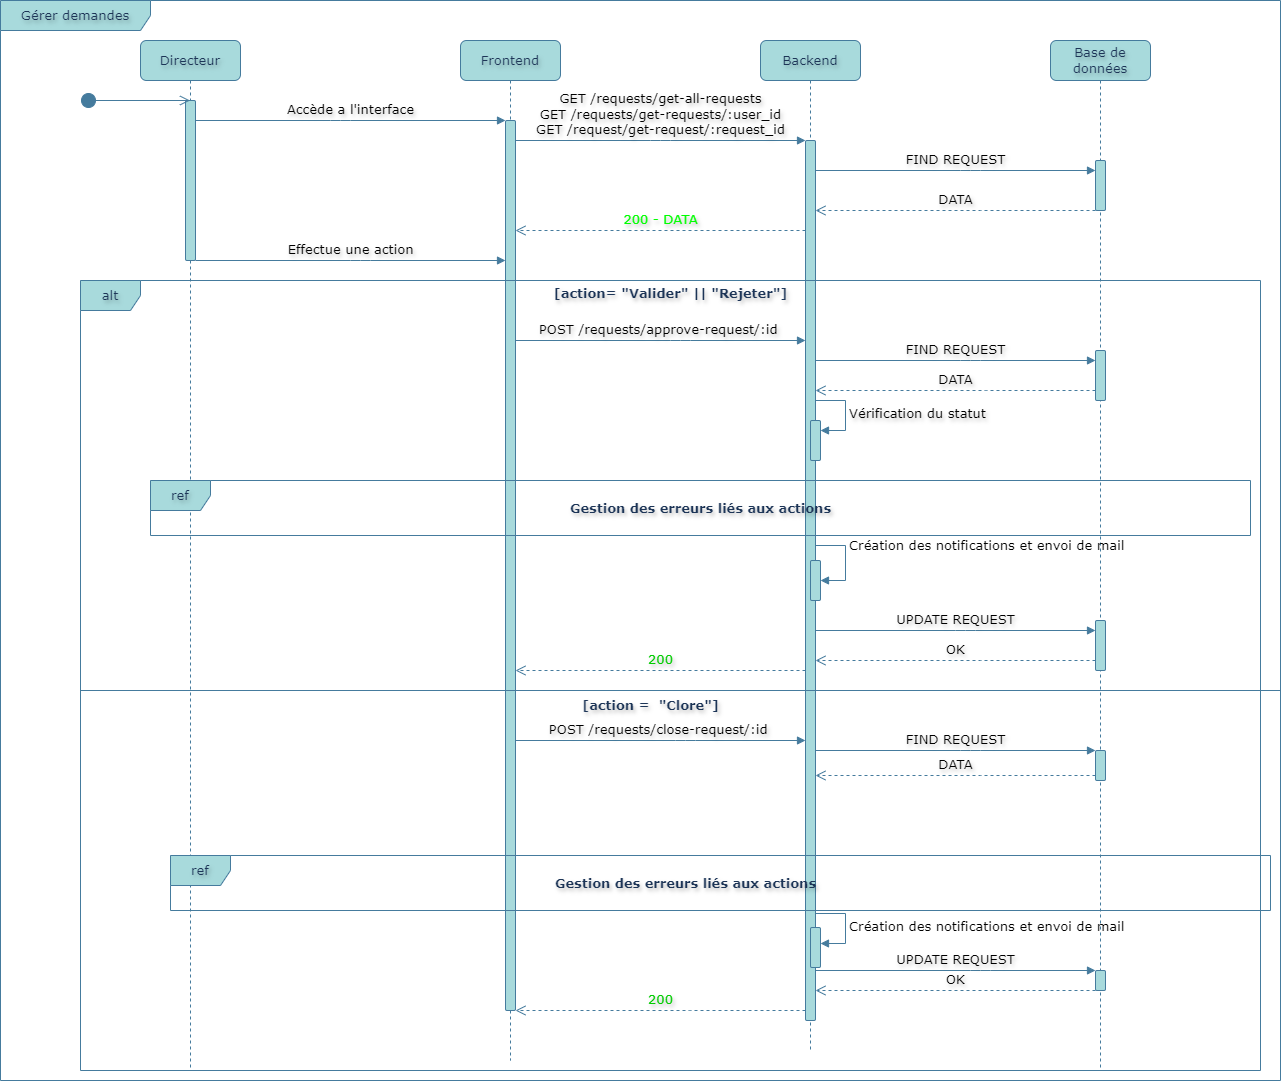
\includegraphics[width=0.9\textwidth]{images/diagramme_de_sequence/gestion_des_demandes_par_le_directeur.drawio.png}
  \caption{Diagramme de séquence - Gestion des demandes par le directeur}
  \label{fig:seq_gestion_demandes}
\end{figure}

\begin{figure}[H]
  \centering
  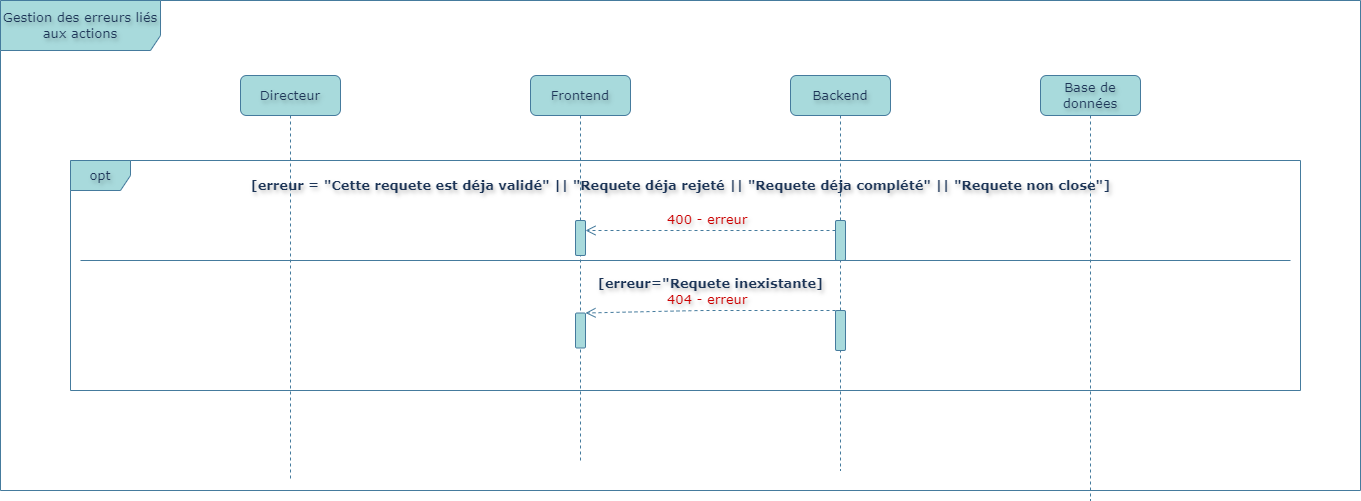
\includegraphics[width=0.9\textwidth]{images/diagramme_de_sequence/gestion_erreurs_demandes.png}
  \caption{Diagramme de séquence - Gestion des erreurs lors du traitement des demandes}
  \label{fig:seq_gestion_erreurs}
\end{figure}

\subsection{Diagramme de séquence « Gestion des demandes par les membres »}

\textbf{Acteur principal :} Membre validé \\
\textbf{Objectif :} Permettre au membre d'éditer, de supprimer et de compléter ses demandes.

\textbf{Scénario principal :}
\begin{enumerate}
  \item Le membre accède à l'interface de gestion des demandes.
  \item Le frontend récupère et affiche les informations relatives aux demandes en effectuant les requêtes suivantes :
  \begin{itemize}
      \item \texttt{GET /requests/get-requests} : obtenir l'historique des demandes effectuées.
      \item \texttt{GET /requests/get-request/:request\_id} : obtenir les détails d'une demande spécifique
  \end{itemize}
  \item Le membre sélectionne une demande et choisit l'action à effectuer :
  
  \textbf{Action : Modifier}
  \begin{itemize}
      \item Le frontend envoie une requête \texttt{PUT /requests/edit-request/:id} au backend avec l'identifiant de la demande et les données à rectifier.
      \item Le backend recherche la demande dans la base de données et vérifie son statut actuel.
      \item \textbf{Cas d'erreur :} Si la demande n'existe pas ou si son statut ne permet pas la modification, le backend retourne un code d'erreur avec un message explicatif. Le frontend affiche ce message au membre.
      \item \textbf{Cas de succès :} Le backend met à jour la demande.
      \item Le backend retourne un code \texttt{200} avec un message de confirmation. Le frontend affiche un message de succès au membre.
  \end{itemize}
  
  \textbf{Action : Compléter}
  \begin{itemize}
      \item Le frontend envoie une requête \texttt{POST /requests/complete-request/:id} au backend avec l'identifiant de la demande.
      \item Le backend recherche la demande dans la base de données et vérifie que son statut permet de la compléter.
      \item \textbf{Cas d'erreur :} Si la demande ne peut pas être complétée (statut incompatible, demande inexistante), le backend retourne un code d'erreur approprié. Le frontend affiche le message d'erreur au membre.
      \item \textbf{Cas de succès :} Le backend marque la demande comme complétée, enregistre l'action et notifie le directeur.
      \item Le backend retourne un code \texttt{200} avec confirmation. Le frontend affiche un message de succès au membre.
  \end{itemize}
  
  \textbf{Action : Supprimer}
  \begin{itemize}
      \item Le frontend envoie une requête \texttt{DELETE /requests/delete-request/:id} au backend avec l'identifiant de la demande.
      \item Le backend recherche la demande dans la base de données et vérifie que son statut permet de la supprimer.
      \item \textbf{Cas d'erreur :} Si la demande ne peut pas être supprimée (statut incompatible, demande inexistante), le backend retourne un code d'erreur approprié. Le frontend affiche le message d'erreur au membre.
      \item \textbf{Cas de succès :} Le backend supprime la demande de la base de données.
      \item Le backend retourne un code \texttt{200} avec confirmation. Le frontend affiche un message de succès au membre.
  \end{itemize}
\end{enumerate}
\begin{figure}[ht]
    \centering
    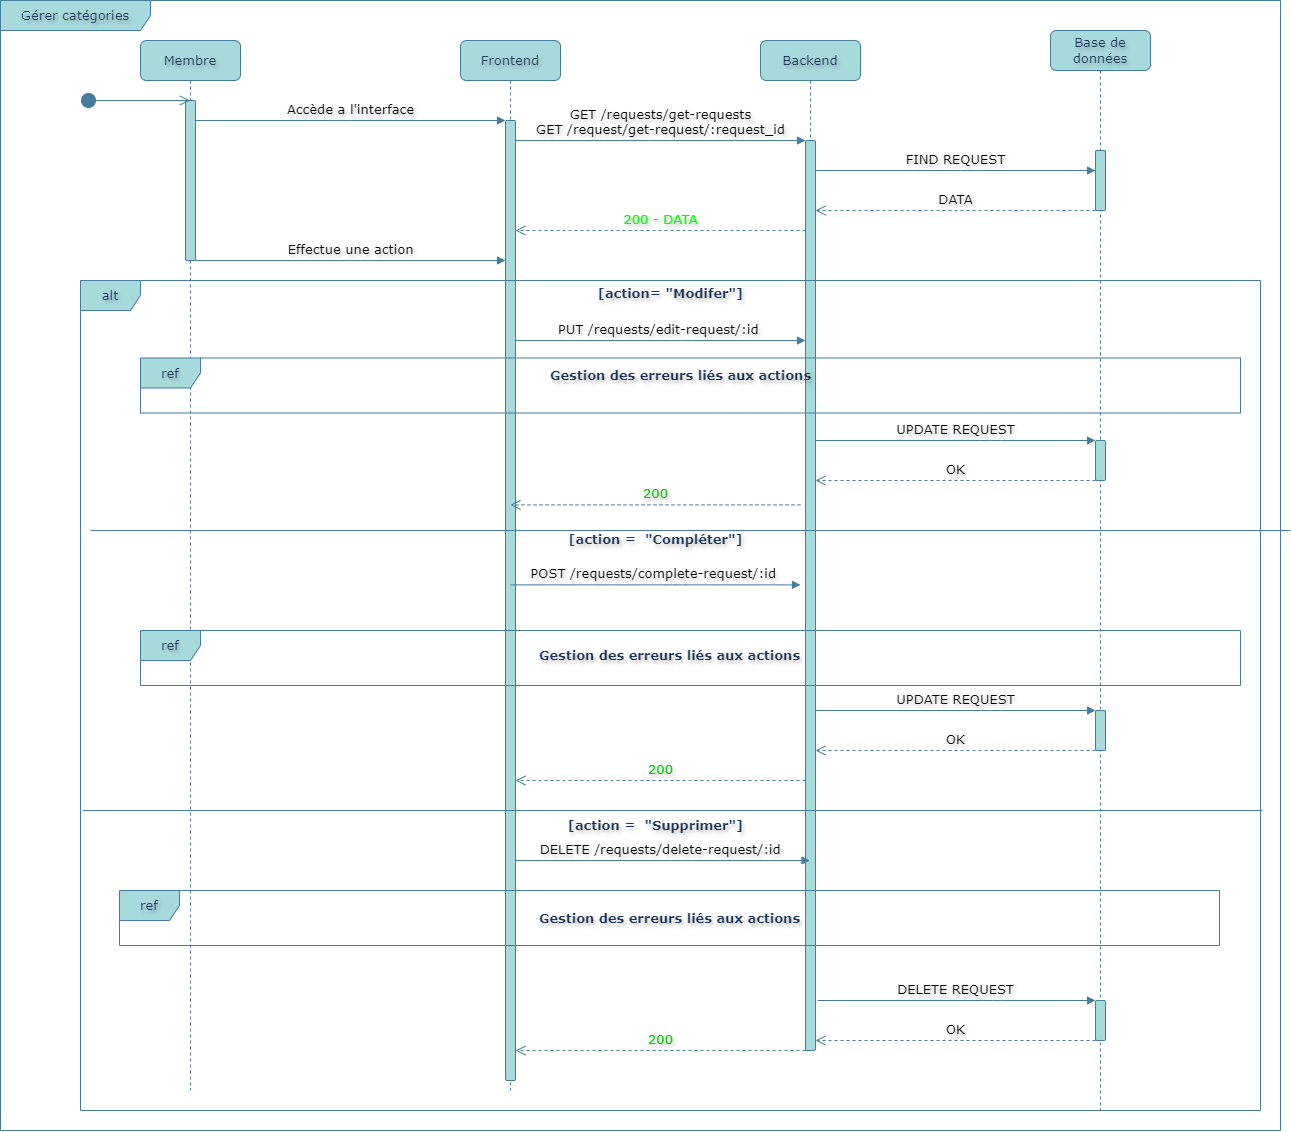
\includegraphics[width=0.9\textwidth]{images/diagramme_de_sequence/gestion_des_demandes_membre.drawio.png}
    \caption{Diagramme de  séquence - Gestion des demandes par les membres}
    \label{fig:demande_diagram}
\end{figure}
\begin{figure}[ht]
    \centering
    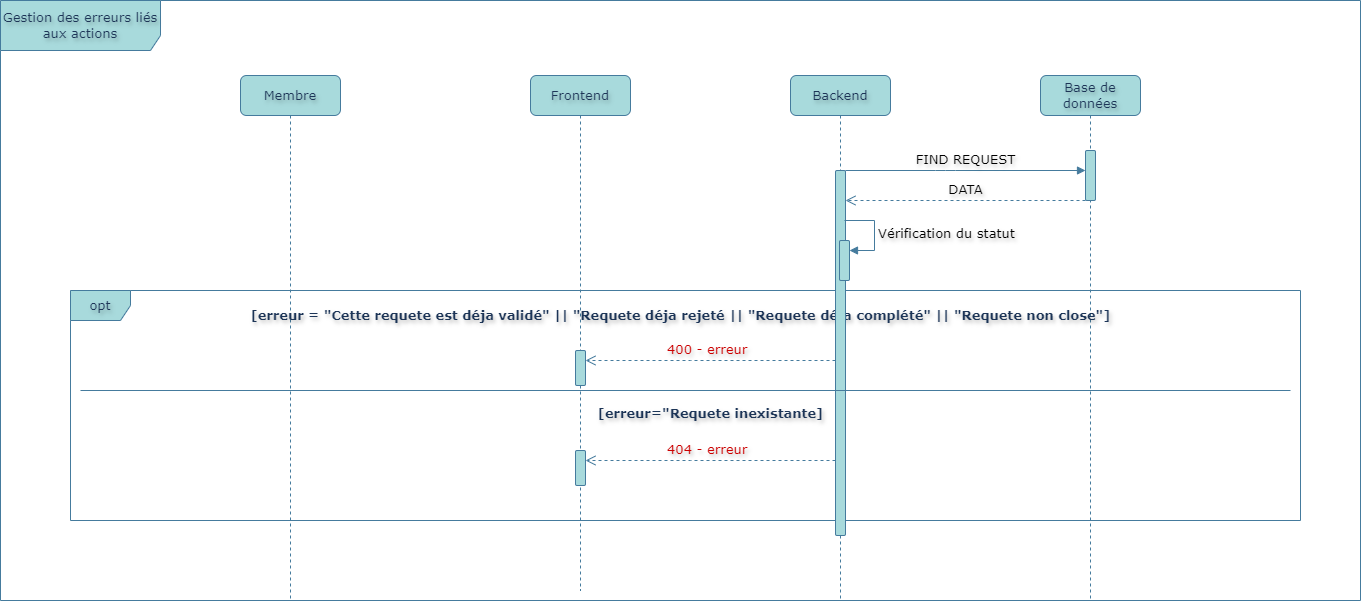
\includegraphics[width=0.9\textwidth]{images/diagramme_de_sequence/gestion_erreurs_demandes_membres.png}
    \caption{Diagramme de  séquence - Gestion des erreurs liés aux actions du membre}
    \label{fig:error_diagram}
\end{figure}


\subsection{Diagramme de séquence « Ajout d'un équipement ou d'une catégorie d'équipement »}

\textbf{Acteur principal :} Directeur \\
\textbf{Objectif :} Enregistrer un équipement ou une catégorie dans le système.

\textbf{Scénario principal :} 
\begin{enumerate}
    \item L'utilisateur accède à l'interface et saisit les informations relatives à l'équipement ou à la catégorie.
    
    \item Le frontend envoie une requête au backend :
    \begin{itemize}
        \item \texttt{POST /equipments/add-equipment} : pour créer un nouveau équipement
        \item \texttt{POST /equipments/add-category} : pour créer une nouvelle catégorie
    \end{itemize}
    
    \item Le backend vérifie qu'un équipement ou une catégorie avec un nom similaire n'existe pas déjà.
    
    \item Le backend retourne une réponse :
    \begin{itemize}
        \item Code \texttt{400} si un équipement ou une catégorie avec un nom similaire existe déjà
        \item Code \texttt{201} si la création a été effectuée avec succès
    \end{itemize}
    
    \item Le frontend affiche le message d'erreur ou de confirmation correspondant à la réponse reçue.
\end{enumerate}

\begin{figure}[H]
  \centering
  \includegraphics[width=0.9\textwidth]{images/diagramme_de_sequence/ajout-equipement-catégorie.drawio.png}
  \caption{Diagramme de séquence - Ajout des équipements et catégories par le directeur}
  \label{fig:seq_ajout_equipement}
\end{figure}



\section{Diagramme de classes}

Le diagramme de classes constitue l’un des éléments centraux de la modélisation UML. Il permet de représenter la structure statique du système ainsi que son architecture orientée objet. Ce diagramme offre une vue d’ensemble des principales classes composant l’application, en détaillant leurs attributs, leurs méthodes et l’ensemble des relations qui les unissent (associations, généralisations, compositions, agrégations, dépendances, etc.).

Cette représentation graphique présente plusieurs avantages majeurs dans le processus de développement :
\begin{itemize}
    \item \textbf{Modélisation conceptuelle} : elle permet de traduire les entités métier du domaine étudié en structures de données cohérentes et réutilisables.
    \item \textbf{Vision architecturale} : elle illustre l’organisation globale du système et facilite la compréhension des interactions entre les différents composants.
    \item \textbf{Guide d’implémentation} : elle constitue une référence technique pour les développeurs lors de la phase de codage.
    \item \textbf{Documentation vivante} : elle sert de support technique actualisable, facilitant ainsi la maintenance évolutive du système.
\end{itemize}

Le diagramme suivant présente la structure complète des classes de notre application, en illustrant les hiérarchies d’héritage, les associations métier ainsi que les cardinalités des relations.

\begin{figure}[H]
    \centering
    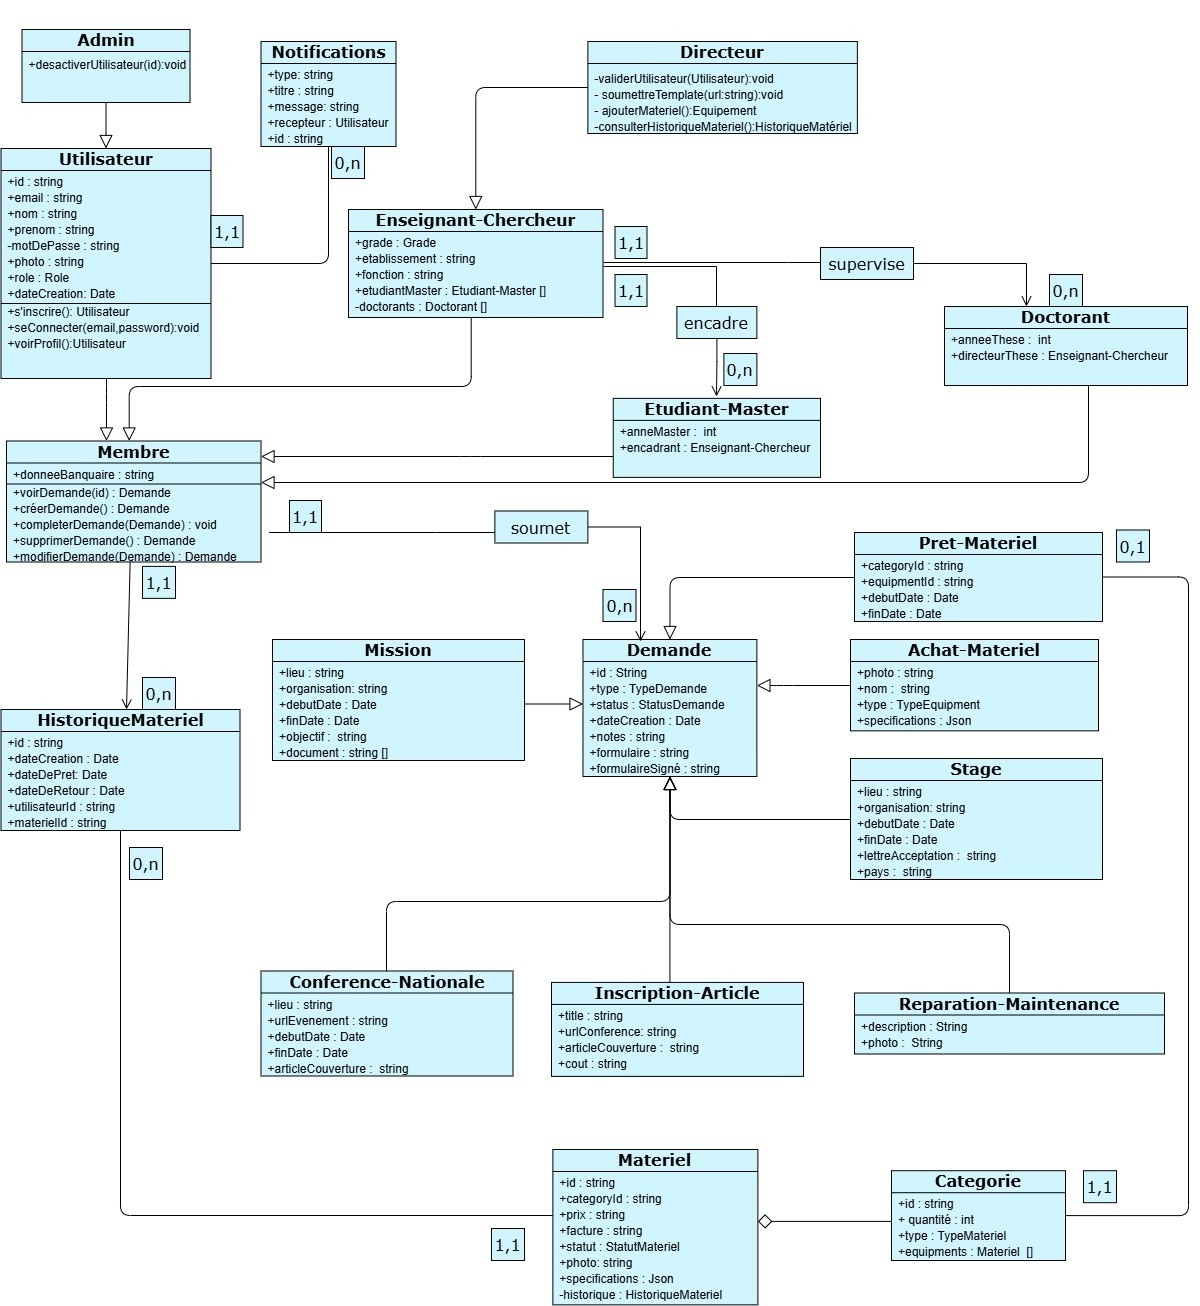
\includegraphics[width=\textwidth]{images/diagramme_de_classe/class.jpg}
    \caption{Diagramme de classes}
    \label{fig:class_diagram}
\end{figure}

\begin{figure}[H]
    \centering
    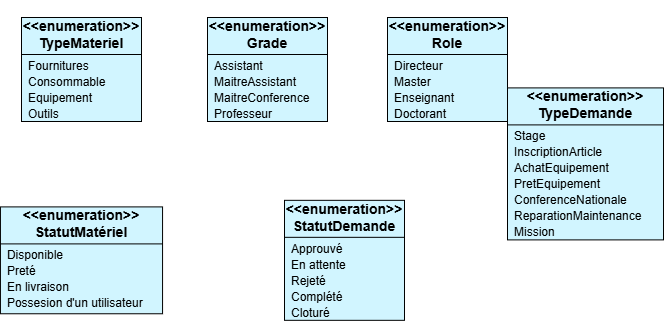
\includegraphics[width=0.7\textwidth]{images/diagramme_de_classe/enums.png}
    \caption{Énumérations utilisées dans le diagramme de classes}
    \label{fig:enum_class}
\end{figure}

Les principales classes modélisées sont les suivantes :

\begin{itemize}
    \item \textbf{Utilisateur} : classe mère des types \textit{Étudiant-Master}, \textit{Doctorant}, \textit{Enseignant-Chercheur}, \textit{Directeur} et \textit{Administrateur}. Elle contient les attributs suivants : \textit{nom, prénom, email, mot de passe, rôle, date de création}.
    
    \item \textbf{Demande} : représente une demande soumise par un utilisateur. Elle contient : \textit{type, description, statut, date, formulaire, formulaire signé}, etc.
    
    \item \textbf{Matériel} : décrit les ressources matérielles disponibles dans le laboratoire.
    
    \item \textbf{Notification} : représente les notifications envoyées automatiquement en fonction des changements de statut des demandes.
\end{itemize}

Les principales relations entre les classes sont :

\begin{itemize}
    \item Un \textbf{Utilisateur} peut soumettre plusieurs \textbf{Demandes}.
    
    \item Un \textbf{Étudiant-Master} ou un \textbf{Doctorant} est encadré par un \textbf{Enseignant-Chercheur}.
\end{itemize}

\section{Résumé}

Dans ce chapitre, nous avons présenté la conception fonctionnelle et structurelle du système via des diagrammes UML. Ces représentations offrent une vue claire des acteurs, des interactions, des processus métier et de l'architecture objet du système. Cette modélisation guidera l'implémentation de la plateforme IRESCOMATH.